\documentclass[12pt]{article}
\usepackage[hmargin=1in,top=1in,bottom=1in]{geometry}

% bibliography stuff
\usepackage{url}
\usepackage{natbib}
\bibpunct[:]{(}{)}{,}{a}{}{,}

% normalem
\usepackage[normalem]{ulem}

% graphics
\usepackage{graphicx}

% tables
\usepackage{longtable}
\usepackage{multirow}
\usepackage{booktabs}

% my example environments
\usepackage{simplex}

% nice feature matrices
\usepackage{amsmath}

% fonts
\usepackage{mathspec}
\setmainfont[Mapping=tex-text]{Linux Libertine}
\setmathfont(Digits,Greek,Latin){Linux Libertine}
%\setmainfont[Mapping=tex-text]{Times New Roman}
%\setmathfont(Digits,Greek,Latin){Times New Roman}

%% KG's shortcuts
\newcommand{\buf}{\hspace{0pt}}
\newcommand{\gap}{\rule{1em}{0.5pt}}
\newcommand{\alt}{\ensuremath{\sim}}
\newcommand{\asp}{\textsuperscript{h}}
\newcommand{\pal}{\textsuperscript{j}}
\newcommand{\zero}{\ensuremath{\emptyset}}
\newcommand{\goesto}{\ensuremath{\longrightarrow}}
\providecommand{\e}[1]{\textsc{e}{$#1$}}

\title{Categorical and gradient aspects of wordlikeness\thanks{Thanks to Gene Buckley, Constantine Lignos, Hilary Prichard, Charles Yang, and audiences at NELS 43 for helpful comments.}}
\author{Kyle Gorman \\ University of Pennsylvania}
\date{Revised January 2013 (comments welcome)}

\begin{document}
\maketitle

\abstract{
Gradient wordlikeness judgements do not necessarily imply that there is a gradient well-formedness system underlying them; gradient judgements may be an artifact of gradient rating tasks.
Dubious architectural assumptions are needed for speakers to report gradient well-formedness judgements.
Simple baselines better account for gradient well-formedness judgements than state-of-the-art computational models of gradient phonotactic knowledge.
}
\section{Introduction}
\chapter{Categorical and gradient aspects of wordlikeness judgements} 
\label{gradience}

Two nonce words, \emph{blick} [blɪk] and \emph{bnick} [bnɪk], underlie the claim that speakers can rapidly distinguish between possible and impossible words \citet{Halle1962}. In \emph{SPE}, \citet{SPE} use a third word, \emph{bnzk}, to argue that nonce words fall on a cline of well-formedness. Neither \emph{bnick} nor \emph{bnzk} are possible words of English, they are possible words in other languages: stop-nasal onsets are found in Moroccan Arabic (e.g., \emph{bniqa} `closet') and stop-nasal-fricative-stop words in Imdlawn Tashlhiyt Berber \citep{Dell1985}. However, there is some sense in which \emph{bnzk} is even less English-like than \emph{bnick}. Of this, \citeauthor{SPE} write:

\begin{quote}
Hence, a real solution to the problem of ``admissibility'' will not simply define a tripartite categorization of occurring, accidental gap, and inadmissible, but will define the `degree of admissibility' of each potential lexical matrix in such a way as to\ldots{}make numerous other distinctions of this sort (\emph{SPE}:416--417)
\end{quote}

\noindent
The position that the well-formedness of nonce words is consistent the view of syntactic grammaticality taken in \emph{LSLT} and \emph{Aspects} \citep{LSLT,ASPECTS}, where it is claimed that different syntactic violations result in different degrees of ungrammaticality.

Most recent discussions of the ``problem of admissibility'' focus on this cline of wellformedness as it is evidenced in wordlikeness tasks.

\begin{quote}
When native speakers are asked to judge made-up (nonce) words, their intuitions are rarely all-or-nothing. In the usual case, novel items fall along a gradient cline of acceptability. \citep[][9]{Albright2009a}

In the particular domain of phonotactics gradient intuitions are pervasive: they have been found in every experiment that allowed participants to rate forms on a scale.
\citep[][382]{Hayes2008a}

\ldots{}when judgements are elicited in a controlled fashion from speakers, they always emerge as gradient, including all intermediate values. \citep[371]{Shademan2006} 
\end{quote}

\begin{quote}
\ldots{}A defect of current grammatical acounts of phonotactics is that they render simple up-or-down decisions concerning well-formedness and cannot account for gradient judgements. \citep[371]{Shademan2006}
\end{quote}

\citet[382]{Hayes2008a} ``consider the ability to model gradient intuitions to be an important criterion for evaluating phonotactic models''.

\begin{quote}
No integer seems to sit on the fence, undecided as to whether it is quite even, or perhaps a bit odd. No odd number seems odder than any other odd number. \citep[274]{Armstrong1983}
\end{quote}

\begin{quote}
Some have responded to these findings very consistently, by asserting that the experimental findings are to be interpreted as before: that, psychologically speaking, odd numbers as well as birds and vegetables are graded concepts\ldots{} We reject this conclusion just because we could not explain how a person could compute with integers who believed that 7 was odder than 23. We assert confidently that the facts about subjects being able to compute and about their being able to give the definition of odd number, etc., are the more important, highly entrenched, facts we want to preserve and explain\ldots{} we ourselves are prepared to give up the seeming fact that some odd numbers appear, as shown by their behavior in certain experimental paradigms, to be odder than others\ldots{}we do not give it up by saying that it was no fact; rather, by saying it must have been a fact about something other than the structure of concepts. \citep[284]{Armstrong1983}
\end{quote}

\begin{quote}
\ldots{}we hold that \emph{fruit} and \emph{odd number} have different structures, and yet we obtain the same experimental outcome for both. But if the same result is achieved regardless of the concept struture, then the experimental design is not pertinent to the determination of concept structure. \citep[284--5]{Armstrong1983}
\end{quote}

At first blush, this would seem to argue against a naïve account of wellformedness judgements in which ill-formedness results when prosodic parsing fails (e.g., \citealt{Ito1989a}, \citealt{Noske1992}, \citealt{OT}). Consider the possibility that a nonce word is ill-formed if it cannot be syllabified without modification. There is a long history for the proposal that impossible words are those whose surface form cannot be parsed into prosodic structures like syllables without further phonological modification (e.g., 

\begin{figure}
\centering
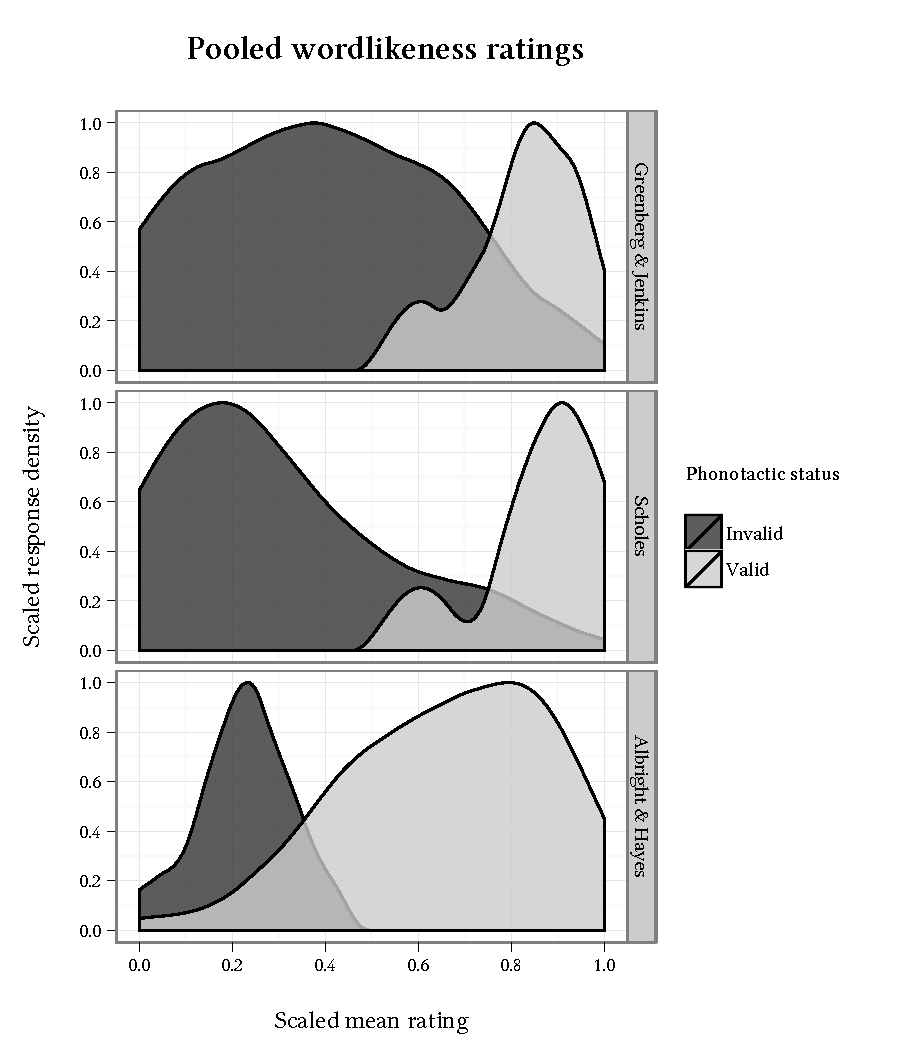
\includegraphics{density.pdf}
\caption{Average ratings of individual nonce words, linearly transformed to fit the interval [0, 1]}
\label{dsn}
\end{figure}

\begin{table}
\centering
\begin{tabular}{l rrr}
\toprule
                        & subjects & items & trials \\
\midrule
\citealt{Albright2007}  & 68       & 40    & 2,720  \\
\citealt{Albright2003a} & 24       & 87    & 2,064  \\
\citealt{Scholes1966}   & 33       & 63    & 2,178  \\
\midrule
\textsc{Total}          & 125      & 187   & 6,962  \\
\bottomrule
\end{tabular}
\caption{Subject and item counts}
\label{counts}
\end{table}

\begin{table}
\centering
\begin{tabular}{l rrrr}
\toprule
Pearson $r$               & \textsc{prosody} & \textsc{maxent} & \textsc{bigram} & \textsc{density} \\
\midrule
\citealt{Albright2007}    & \textbf{.725}    & {.703}          & {.463}          & {.695}           \\
\citealt{Albright2003b}   & {.594}           & {.208}          & \textbf{.746}   & {.688}           \\
\citealt{Scholes1966}     & {.803}           & {.534}          & {.737}          & \textbf{.834}    \\
\midrule
Spearman $\rho$           & \textsc{prosody} & \textsc{maxent} & \textsc{bigram} & \textsc{density} \\
\midrule
\citealt{Albright2007}    & \textbf{.819}    & {.661}          & {.338}          & {.612}           \\
\citealt{Albright2003b}   & {.662}           & {.389}          & {.699}          & \textbf{.739}    \\
\citealt{Scholes1966}     & {.769}           & {.575}          & {.794}          & \textbf{.817}    \\
\midrule
Kendall $\tau_{b}$        & \textsc{prosody} & \textsc{maxent} & \textsc{bigram} & \textsc{density} \\
\midrule
\citealt{Albright2007}    & {.666}           & \textbf{.683}   & {.245}          & {.450}           \\
\citealt{Albright2003b}   & {.474}           & {.159}          & {.499}          & \textbf{.558}    \\
\citealt{Scholes1966}     & {.619}           & {.484}          & {.614}          & \textbf{.671}    \\
\midrule
Goodman-Kruskal $\gamma$  & \textsc{prosody} & \textsc{maxent} & \textsc{bigram} & \textsc{density} \\
\midrule
\citealt{Albright2007}    & \textbf{.874}    & {.849}          & {.502}          & {.574}           \\
\citealt{Albright2003b}   & \textbf{.929}    & {.606}          & {.246}          & {.488}           \\
\citealt{Scholes1966}     & \textbf{.907}    & {.558}          & {.628}          & {.738}           \\
\bottomrule
\end{tabular}
\caption{FIXME}
\label{scores}
\end{table}

%\subsubsection{Maximum entropy phonotactics}
%
%\citeauthor{Hayes2008a} (\citeyear{Hayes2008a}; henceforth H\&W) develop a sophisticated model of phonotactic grammaticality which estimates a probability distribution over phoneme sequences by weighing constraints according to the principle of maximum entropy, following \citet{Goldwater2003} and \citet{Jager2007}. H\&W report that the predictions of their model are closely correlated with the \citet{Scholes1966} wordlikeness ratings. A direct replication of their predictions was attempted by using the software, model parameters, and training data as described in that study. Since the training of the maximum entropy model is inherently stochastic, producing slightly different outcomes on each run, the lowest scoring of ten runs is reported (H\&W:396), though in general there is not a great deal of variation between individual runs. One limitation of this model is that it is not feasible to score whole words, as the number of constraints which must be inspected grows exponentially as the span of possible constraints increases. Following H\&W and of \citet{Albright2009a}, who also applies the maximum entropy model to the \citet{Albright2003b} norms, the model is trained and scored only on stimulus onsets. However, as a consequence, the maximum entropy model performs particularly poorly on this data set, as many stimuli contain phonotactic violations in rime positions.
%
%\subsubsection{Segment bigram probability} 
%\label{bigram}
%
%The bigram probability of a sequence $ijk$ is the product of the probability of an sequence-initial $i$, the probability that $j$ follows $i$, and the probability that $k$ follows $j$, and the product of sequence-final \emph{k}.
%
%\begin{unlabeledexample}
%$\displaystyle \hat{p}(ijk) = p(i|\textrm{start}) \cdot p(j|i) \cdot p(k|j) \cdot p(\textrm{stop}|k)$
%\end{unlabeledexample}
%
%\noindent \citet{Albright2009a} employs bigram probability to model wordlikeness judgements. While the focus of \citeauthor{Albright2009a}'s study is on developing a model which uses bigrams over phonological features rather than segments themselves, \citeauthor{Albright2009a}'s evaluation, which includes both the \citeauthor{Scholes1966} and \citeauthor{Albright2003b} data sets, finds an advantage for segmental bigrams. \citeauthor{Albright2009a} does not provide an implementation of the featural bigram model, nor does his study describe it in sufficient detail to allow for a new implementation, but segmental bigram scores for the \citeauthor{Albright2003a} data are reported in the appendix. As reported by \citeauthor{Albright2009a}, segmental bigrams outperform featural bigrams (see Table \ref{albrightimproved}).
%
%\citeauthor{Albright2009a} estimates bigram probabilities using the method of maximum likelihood over types in the lexicon. The variant of segmental bigrams used here computes probabilities with a simple type of smoothing in which the count of all possible bigrams (including those never observed) are incremented by one. This technique is known as Laplace, or ``add one'' smoothing. This has the desirable effect that no nonce word is ever assigned a zero probability, and produces a small increase in the correlation between the \citeauthor{Albright2003b} wordlikeness norms compared with the maximum likelihood estimate (Table \ref{albrightimproved}). For all three data sets, this model also consistenly outperforms positional probability models defined by \citet{Vitevitch2004} and \citet{Vaden2009}; given that these model scores are highly correlatd with bigram probability \citep[][54]{Vitevitch1997}, they are not considered further. The bigram model consistently performs well in all the evaluations, and has the highest Spearman correlation with the \citeauthor{Greenberg1964} and \citeauthor{Scholes1966} data, and is frequently second place model to the binary baseline elsewhere.
%
%\subsubsection{Neighborhood density} 
%\label{density}
%
%There are now many methods for computing similarity between nonce words and existing words, long thought to be reflected in wordlikeness judgements. 
%For this study, a number of such methods were evaluated, including the Generalized Neighborhood Model \citep{Bailey2001}, PLD20 \citep{Suarez2011}, and a number of variations on neighborhood density \citep{Coltheart1977} provided by \citet{Vaden2009}. The best performance was obtained with the simplest version of neighborhood density, which is defined as the number of real monomorphemic words which can be changed into the target nonce word by a single insertion, deletion, or substitution of a phone.\footnote{\citet{Greenberg1964} use a variant in which only substitutions are counted.} For instance, the neighbors of \emph{blick} include \emph{blink} (insertion), \emph{lick} (deletion) and \emph{black} (substitution). While many studies \citep[e.g.,][]{Bailey2001} report robust lexical similarity effects, it may be that the relatively weak performance of neighborhood density is the result of the presence of gross phonotactic violations.
%
%\subsection{Modeling residual gradience}
%
%The primary result is that no gradient model reliably exceeds the accuracy of the binary baseline. Despite this, there are relatively strong correlations between the binary baseline and these gradient models (see Table \ref{bcor}). From the strong performance of the categorical model one can infer that the gradient models do not reliably predict intermediate ratings, or contrasts in ratings between words which are grouped together. To quantify this, the following method was used to estimate the residual contribution of the three gradient models once gross phonotactic violations are taken into account. Instead of calculating rank correlations directly on the model scores as in Table \ref{cor}, the model scores are mapped to ranks with the additional constraint that all ``valid'' stimuli be ranked above all ``invalid'' stimuli. The resulting ranks are used to compute new correlation statistics. Finally, the binary baseline correlation is subtracted from this number, so that the resulting value is the amount of improvement derived from augmenting the binary model with gradience. These difference numbers are shown in Table \ref{controlled}. In most cases, including the gradient models on top of the binary baseline produces a worse correlation than is obtained with the binary baseline alone.
%
%For $\tau_b$ and $\gamma$, the interpretation of this result is clear. The gradient models assign rankings to the sets of phonotactically valid and invalid clusters, respectively. For instance, the bigram model favors \emph{troog} [tɹuːɡ] over \emph{swach} [swætʃ], though neither contains any gross phonotactic violation. Similarly, the bigram model favors \emph{chwoop} [tʃwuːp] over \emph{zhrick} [ʒɹɪk], even though both contain ill-formed onsets. However, the majority of such predicted contrasts are not reflected in speakers' judgements; for instance, \emph{troog} is rated less English-like than \emph{swach} \citep{Greenberg1964}, contrary to the model predictions. This shows quite starkly that these models fail to reliably predict intermediate ratings.
%
%\subsection{The gradience hypothesis}
%
%This chapter has evaluated the axiom of gradience as a falsifiable alternative hypothesis. The surprising result is that virtually all of the apparent coverage of state-of-the-art gradient phonotactic models is simply a reflection of their ability to distinguish between the possible and the totally impossible; beyond this, they are unreliable. A trivial baseline, endowed with few abilities to project beyond the observed data, generally outperforms the state of the art. The projections made by the state-of-the-art gradient models are not like those made by speakers. It remains to be seen is whether any model can be put forth which accurately predicts these intermediate ratings.
%
%These result provide support for recent findings that speakers asked to perform gradient syntactic judgements produce responses closely corresponding to a widely recognized categorical grammatical/ungrammatical distinction \citep{Sprouse2007}.
%
%\subsection{Extensions to the binary baseline}
%
%The strong performance of the binary baseline should not be taken as evidence either that wordlikenesss judgements are binary, or that the binary baseline is a plausible model. The most serious limitation of this evaluation is the primitive nature of the binary baseline. The inability to generalization within onsets and rimes is a serious flaw, as is the assumption of independence of onset and rime. Regarding the rime, \citet{Borowsky1989} proposes a theory of possible rimes in English, which does make the correct prediction regarding the unattested but well-formed [ɛsp]. On the other hand, a cognitively plausible version of this model might need to entertain phonotactic generalizations that are larger than these units, since syllable-sized phonotactic generalizations have been proposed for English \citep[e.g.,][]{Berkley1994a,Berkley1994b,Coetzee2008b,Fudge1969}. 
%
%A possible further extension to the binary baseline would be the introduction of additional levels of wellformedness. While the evaluation has shown that current gradient models do not reliably identify intermediate wellformedness, it does seem possible to identify at least three levels of grammaticality: for instance, one might encode the intuition that \emph{zhlick} [ʒlɪk] is more English-like than \emph{bnick}, though both have unattested onsets. There are precedents for labeling certain attested words as phonotactically ``peripheral'' (see, e.g., the appendices in \citealt{Myers1987} and \citealt{Borowsky1989}); such words are regarded as lexical exceptions to language-general principles of syllabification. If this extends to nonce words, then an intermediate level of grammaticality could be assigned to ``possible'' but formally marked words. Another likely source of additional levels of grammaticality is the cumulative effect of multiple phonotactic violations. While, as \citet{Coleman1997} note, classical Optimality Theory predicts that a nonce word is as ill-formed as its worst deviation from syllable structure, it is possible to imagine that multiple phonotactic violations would result in greater degrees of ill-formedness. The bigram and maxent models make this prediction, as do many others \citep[e.g.,][]{Legendre1990,Levelt2000,Albright2008,Anttila2008a,Pater2009b} but despite this, there is still little data demonstrating cumulative effects in wordlikeness tasks.
%
%\subsection{Language acquisition}
%
%The weak empirical status of gradient phonotactic knowledge as reflected in adults has rammifications for language acquisition under the hypothesis that that infants acquiring language deploy the same representations as adults \citep[e.g.,][]{Macnamara1982,Pinker1984,Crain1991,Carey1995,deVilliers2001,Legate2007}. Gradient wordlikeness judgements in adults would provide support for claims that infants recognize statistical(inherently gradient) dependencies between segments \citep{Jusczyk1994} and use these to segment words \citep{Saffran1996}. An emerging consensus suggests, however, that infants attend to transitional probabilities primarily in the absence of grammatical cues \citep{Gambell2005,Hohne1994,Johnson2001,Jusczyk1999c,Lignos2012b,Mattys2001a,Shukla2007,Lew-Williams2012}. The vacuous nature of current evidence for gradient phonotactic knowledge in adults further weakens any hypothesis that would link statistical learning in infants to adults' behaviors.
%
%\section{Conclusion}
%
%%For instance, infants as young as 4.5 months seem to be aware that English nasal codas agree in place with following obstruents \citep{Mattys2001b,Jusczyk2002,Davidson2004}. 
%%It might be the case that syllable co-occurrence statistics might be little more than a reflection of infants' learning of categorical ``lexical viability'' constraints \citep{Johnson2003} of the sort also seen in adult speech processing \citep[e.g.,][]{Norris1997}. 
%
%% other ratings, but por qué?:
%% 
%% Hayes2000
%% 
%% Albright2003a
%% Albright2003b
%% Prasada1993 
%% 
%% Bard1996
%% 
%% Koo2009
%% 
%% Treiman2000
%% 
%% Warker2006
%% 
%% Massaro1983
%% 
%% Rusaw2009
%do not explicitly state why this data is relevant to the construction of models of wordlikeness. Presumably, these authors believe that these patterns of judgements demonstrate that wordlikeness, as an internal state, is gradient simply because subjects make use of intermediate degrees of wordlikeness in judgement tasks. This proposition, generalized below, is ``naïve'' not because it lacks sophistication, but because it is rooted in a belief in naïve realism, a philosophy which holds that perception provides a relatively direct picture of the nature of the world, an influential view in the cognitive sciences in general (see \citealt{Fodor1981a} for a critique).
%
%\citeauthor{Chomsky1965} were not the first to consider the notion of possible and impossible words. Their primary contribution is that their mentalist perspective: they recognize that naïve speakers effortlessly acquire language-specific generalizations about possible and impossible words and can report them without any explicit training.
%
%However, not all early literature is concerned with gradience. \citet[31]{Vogt1954}, for instance, recognizes that the taxonomic phoneme is insufficient to account for many wordlikeness contrasts. \citeauthor{Vogt1954} observes that allophony may account for the absence of certain phone sequences, but it does not provide a suitable explanation for the absence of initial [bn] in English, nor does it make correct predictions about the surface realization of an underlying initial /bn/. \citeauthor{Vogt1954} concludes that additional grammatical machinery will be needed to account for possible and impossible words. 
%
%Most relevant to the question at hand, \citet{Frisch2000} and \citet{Vitevitch1997} find that speakers' wordlikeness ratings of multisyllabic words are correlated wtih the positional probailities of the constituent syllables. Unfortunately, none of these researchers make any effort to eliminate the possibility that the low positional probability stimuli are ``impossible'' words of English. In fact, 
%Chapter \ref{clusters} argues
%%the author has argued elsewhere \citep{Gorman2012c}
%that many of the stimuli used by \citeauthor{Frisch2000} and \citeauthor{Vitevitch1997} contain illicit word-medial consonant clusters. While \citeauthor{Vitevitch1997} neither control nor manipulate the well-formedness of medial clusters, in a post-hoc test they consider a probabilistic measure of cluster well-formedness, which reveals that cluster well-formedness is correlated with syllable-internal positional probabilities and wordlikeness judgements, but \citeauthor{Vitevitch1997} ultimately conclude this cannot explain all the variation in wordlikeness. 
%
%Using the head-term preference paradigm, \citet{Jusczyk1993b} and \citet{Friederici1993} find that typically-developing children as young as 9 months of age distinguish between nonce words which are and are not phonotactically valid in their target language. \citet{Jusczyk1994} report that 9-month-old children acquiring English also show preferences for nonce words with high positional probability over those with low positional probability. Faciliatory effects of positional probability (i.e., shorter latencies) are reported for other nonce word tasks conducted with adults, including single-word shadowing \citep{Vitevitch1997,Vitevitch1998}, same/different judgements \citep{Vitevitch1999a,Luce2001,Lipinski2005,Vitevitch2005}, and lexical decision \citep{Pylkkanen2002a}.
%
%The aforementioned studies all conclude that the gradient measure of positional probability correlates with behavioral results. As the flaws of the \citet{Vitevitch1997} study demonstrate, the aforementioned studies do little to tease apart the gradient and categorical aspects of phonotactics. More generally, they do little to distinguish between positional probability and closely correlated measures like bigram probability (see \S\ref{bigram} below) or neighborhood density, since these studies carefully select stimuli which either have high or low values for all of positional probability, bigram probablility, and neighborhood density. This is particularly troublesome given that no justification has ever been given for the positional probability measure in the first place; it appears to have been created \emph{ex nihilo}; in contrast, the effects of neighborhood density in various psycholinguistic tasks are emergent properties of many models of speech production \citep[e.g.,][]{Luce1998,Luce2000} and perception \citep{Marslen-Wilson1984,Marslen-Wilson1987,McClelland1986,Norris1994,Norris2000}. 
%\subsubsection{\citealt{Greenberg1964}}
%
%\citet{Greenberg1964} investigated wordlikeness using the technique of free magnitude estimation, a mechanism which has become increasingly popular among syntacticians \citep[e.g.,][]{Bard1996}. At the beginning of the experiment, the subject heard a recording of the word \emph{stick}. In subsequent trials, the subjects heard a nonce word and were asked to report ``how far would you say that is from English?'', with \emph{stick} at ``1''; subjects are told that a word that is ``twice as far from English'' as \emph{stick} should be scored ``2''. The data used here are from \citeauthor{Greenberg1964}'s Experiment B, in which 17 undergraduates were presented 17 stimuli in all. In addition to \emph{stick}, the stimuli include three other English words; these four items were excluded from further analyses, leaving 13 stimuli. As is standard practice in psychophysics \citep[e.g.,][]{Butler1987}, magnitudes were log-transformed prior to analysis.
%


\appendix
\renewcommand{\arraystretch}{0.25}
\section{English wordlikeness ratings}
\label{ratings}

\subsection{\citet{Albright2007}}

\begin{longtable}{r@{ }r@{ }c@{ }l@{ }l rrrrrr}
\toprule
   &   &     &   &    & lexical & $-$log $p$ & $-$log $p$ & gross  & rating    \\
   &   &     &   &    & density & (bigram)   & (MaxEnt)   & status & (7-point) \\
\midrule
P & L & IY1 & N &    & 13 & 13.585 & 0.000 &   valid & 5.32 \\
B & L & AA1 & D &    & 13 & 17.609 & 0.000 &   valid & 5.13 \\
P & L & IY1 & K &    & 11 & 14.200 & 0.000 &   valid & 5.06 \\
P & L & EY1 & K &    & 14 & 15.576 & 0.000 &   valid & 4.94 \\
P & R & AH1 & N & JH & 3 & 16.546 & 0.000 &   valid & 4.94 \\
B & L & UW1 & T &    & 14 & 15.692 & 0.000 &   valid & 4.84 \\
P & L & IH1 & M &    & 5 & 15.126 & 0.000 &   valid & 4.71 \\
B & L & EH1 & M &  P & 1 & 19.447 & 0.000 &   valid & 4.69 \\
B & L & AH1 & S &    & 14 & 13.806 & 0.000 &   valid & 4.67 \\
B & L & AE1 & D &    & 15 & 16.259 & 0.000 &   valid & 4.65 \\
B & L & IH1 & G &    & 4 & 16.347 & 0.000 &   valid & 4.58 \\
P & R & EH1 & S &  P & 4 & 17.214 & 0.000 & invalid & 4.50 \\
B & R & EH1 & N & TH & 4 & 21.255 & 0.000 &   valid & 4.11 \\
P & R & AH1 & P &  T & 4 & 18.487 & 0.000 &   valid & 4.07 \\
B & R & EH1 & L & TH & 2 & 23.014 & 0.000 &   valid & 3.14 \\
P & W & IH1 & S &  T & 4 & 21.499 & 0.000 &   valid & 2.94 \\
B & W & AH1 & D &    & 2 & 20.596 & 0.000 &   valid & 2.94 \\
B & W & AA1 & D &    & 3 & 21.329 & 0.000 &   valid & 2.94 \\
P & W & AE1 & D &    & 2 & 24.103 & 0.000 &   valid & 2.89 \\
P & W & AH1 & S &    & 4 & 20.684 & 0.000 &   valid & 2.61 \\
P & W & EH1 & T &    & 6 & 20.998 & 0.000 &   valid & 2.53 \\
P & T & IY1 & N &    & 4 & 15.440 & 6.762 & invalid & 2.44 \\
B & W & AE1 & D &    & 2 & 23.365 & 0.000 &   valid & 2.41 \\
B & N & IY1 & N &    & 2 & 21.180 & 7.296 & invalid & 2.39 \\
P & W & AH1 & D &  Z & 0 & 25.210 & 0.000 &   valid & 2.17 \\
P & N & IY1 & N &    & 2 & 21.181 & 6.019 & invalid & 2.16 \\
B & N & AH1 & S &    & 6 & 19.732 & 7.296 & invalid & 2.06 \\
P & N & EH1 & P &    & 2 & 23.587 & 6.019 & invalid & 2.00 \\
B & N & AA1 & D &    & 2 & 24.066 & 7.296 & invalid & 2.00 \\
B & Z & IY1 & N &    & 1 & 16.896 & 19.097 & invalid & 2.00 \\
P & T & AH1 & S &    & 3 & 14.169 & 6.762 & invalid & 1.94 \\
P & T & EH1 & P &    & 3 & 17.228 & 6.762 & invalid & 1.86 \\
B & Z & AH1 & S &    & 2 & 15.237 & 19.097 & invalid & 1.81 \\
P & N & IY1 & K &    & 2 & 21.796 & 6.019 & invalid & 1.76 \\
B & D & IY1 & K &    & 2 & 18.773 & 13.131 & invalid & 1.72 \\
B & D & UW1 & T &    & 3 & 19.781 & 13.131 & invalid & 1.71 \\
B & D & AH1 & S &    & 4 & 17.041 & 13.131 & invalid & 1.71 \\
P & T & AE1 & D &    & 3 & 17.622 & 6.762 & invalid & 1.67 \\
B & Z & AA1 & D &    & 1 & 20.151 & 19.097 & invalid & 1.63 \\
B & Z & AY1 & K &    & 1 & 19.118 & 19.097 & invalid & 1.28 \\
\bottomrule
\end{longtable}

\subsection{\citet{Albright2003b}, norming study} 

\begin{longtable}{r@{ }r@{ }r@{ }c@{ }l@{ }l@{ } rrrrr}
\toprule
   &    &    &    &    &   & lexical & $-$log $p$ & $-$log $p$ & gross  & rating    \\
   &    &    &    &    &   & density & (bigram)   & (MaxEnt)   & status & (7-point) \\
\midrule
  &  S &  L & EY1 & M  &    & 15 & 17.469 & 0.000 &   valid & 5.84 \\
  &    &  W & IH1 & S  &    & 34 & 11.208 & 0.000 &   valid & 5.84 \\
  &    &  P & IH1 & N  & T  & 26 & 13.046 & 0.000 &   valid & 5.67 \\
  &    &  P & AE1 & NG & K  & 18 & 13.723 & 0.000 &   valid & 5.63 \\
  &  S &  T & IH1 & P  &    & 18 & 12.599 & 0.000 &   valid & 5.53 \\
  &    &  M & IH1 & P  &    & 33 & 12.345 & 0.000 &   valid & 5.47 \\
  &  S &  T & AY1 & R  &    & 11 & 15.118 & 0.000 &   valid & 5.47 \\
  &    &  M & ER1 & N  &    & 34 & 12.872 & 0.000 &   valid & 5.42 \\
  &  P &  L & EY1 & K  &    & 14 & 15.576 & 0.000 &   valid & 5.39 \\
  &  S &  N & EH1 & L  &    & 10 & 18.582 & 0.000 &   valid & 5.32 \\
  &  S &  T & IH1 & N  &    & 18 & 10.899 & 0.000 &   valid & 5.28 \\
  &    &  R & AE1 & S  & K  & 11 & 15.544 & 0.000 &   valid & 5.21 \\
  &  T &  R & IH1 & S  & K  &  5 & 17.980 & 0.000 &   valid & 5.21 \\
  &  S &  P & AE1 & K  &    & 17 & 14.205 & 0.000 &   valid & 5.16 \\
  &    &  D & EY1 & P  &    & 22 & 14.193 & 0.000 &   valid & 5.11 \\
  &    &  G & EH1 & R  &    & 25 & 13.044 & 0.000 &   valid & 5.11 \\
  &  G &  L & IH1 & T  &    & 14 & 16.830 & 0.000 &   valid & 5.11 \\
  &  S &  K & EH1 & L  &    & 16 & 16.356 & 0.000 &   valid & 5.11 \\
  &    & SH & ER1 & N  &    & 23 & 15.913 & 0.000 &   valid & 5.11 \\
  &    &  T & AA1 & R  & K  & 18 & 17.702 & 0.000 &   valid & 5.11 \\
  &    & CH & EY1 & K  &    & 28 & 15.023 & 0.000 &   valid & 5.05 \\
  &  G &  L & IY1 & D  &    & 14 & 16.118 & 0.000 &   valid & 5.05 \\
  &  G &  R & AY1 & N  & T  &  4 & 17.626 & 0.000 &   valid & 5.00 \\
  &  P &  R & IY1 & K  &    & 11 & 13.396 & 0.000 &   valid & 5.00 \\
  &    & SH & IH1 & L  & K  &  8 & 21.270 & 0.000 &   valid & 4.89 \\
  &    &  D & AY1 & Z  &    & 39 & 12.730 & 0.000 &   valid & 4.84 \\
  &    &  N & EY1 & S  &    & 23 & 14.952 & 0.000 &   valid & 4.84 \\
  &    &  T & AH1 & NG & K  & 18 & 15.046 & 0.000 &   valid & 4.84 \\
S &  K &  W & IH1 & L  &    &  6 & 18.210 & 0.000 &   valid & 4.83 \\
  &    &  L & AH1 & M  &    & 35 & 11.569 & 0.000 &   valid & 4.79 \\
  &    &  P & AH1 & M  &    & 30 & 11.121 & 0.000 &   valid & 4.79 \\
S &  P &  L & IH1 & NG &    & 14 & 15.573 & 0.000 &   valid & 4.72 \\
  &  G &  R & EH1 & L  &    &  3 & 14.624 & 0.000 &   valid & 4.63 \\
  &    &  T & EH1 & SH &    & 12 & 14.517 & 0.000 &   valid & 4.63 \\
  &    &  T & IY1 & P  &    & 32 & 12.980 & 0.000 &   valid & 4.63 \\
  &    &  B & AY1 & Z  &    & 35 & 12.821 & 0.000 &   valid & 4.58 \\
  &  G &  L & IH1 & P  &    & 11 & 17.377 & 0.000 &   valid & 4.53 \\
  &    & CH & AY1 & N  & D  & 18 & 17.747 & 0.000 &   valid & 4.37 \\
  &  P &  L & IH1 & M  &    &  5 & 15.126 & 0.000 &   valid & 4.37 \\
  &    &  G & UW1 & D  &    & 29 & 15.448 & 0.000 &   valid & 4.32 \\
  &  B &  L & EY1 & F  &    &  6 & 19.485 & 0.000 &   valid & 4.21 \\
  &    &  G & EH1 & Z  &    & 17 & 16.466 & 0.000 &   valid & 4.21 \\
  &  D &  R & IH1 & T  &    &  8 & 15.563 & 0.000 &   valid & 4.16 \\
  &  F &  L & IY1 & P  &    & 10 & 15.292 & 0.000 &   valid & 4.16 \\
  &    &  Z & EY1 &    &    & 23 & 15.208 & 0.000 &   valid & 4.16 \\
S &  K &  R & AY1 & D  &    &  5 & 18.722 & 0.000 &   valid & 4.11 \\
  &    &  K & IH1 & V  &    & 16 & 12.591 & 0.000 &   valid & 4.05 \\
  &  F &  L & EH1 & T  &    & 17 & 16.490 & 0.000 &   valid & 4.00 \\
  &    &  N & OW1 & L  & D  & 19 & 19.101 & 0.000 &   valid & 4.00 \\
  &  S &  K & IH1 & K  &    & 13 & 14.628 & 0.000 &   valid & 4.00 \\
  &  B &  R & EH1 & JH &    &  7 & 17.318 & 0.000 &   valid & 3.95 \\
  &  K &  W & IY1 & D  &    & 10 & 16.039 & 0.000 &   valid & 3.95 \\
  &  S &  K & OY1 & L  &    &  9 & 19.350 & 0.000 &   valid & 3.89 \\
  &  D &  R & AY1 & S  &    & 12 & 17.758 & 0.000 &   valid & 3.84 \\
  &  F &  L & IH1 & JH &    &  8 & 17.312 & 0.000 &   valid & 3.79 \\
  &  B &  L & IH1 & G  &    &  4 & 16.347 & 0.000 &   valid & 3.53 \\
  &    &  Z & EY1 & P  & S  &  7 & 24.825 & 0.000 &   valid & 3.47 \\
  &    & CH & UW1 & L  &    & 17 & 14.492 & 0.000 &   valid & 3.42 \\
  &    & SH & AY1 & N  & T  &  8 & 18.503 & 0.000 &   valid & 3.42 \\
  & SH &  R & UH1 & K  & S  &  5 & 26.733 & 0.000 &   valid & 3.32 \\
  &  G &  W & EH1 & N  & JH &  0 & 22.722 & 0.000 &   valid & 3.32 \\
  &    &  N & AH1 & NG &    & 19 & 15.754 & 0.000 &   valid & 3.28 \\
S &  K &  W & AA1 & L  & K  &  1 & 25.752 & 0.000 & invalid & 3.26 \\
  &  T &  W & UW1 &    &    &  5 & 17.918 & 0.000 &   valid & 3.17 \\
  &  S &  M & AH1 & M  &    &  8 & 14.940 & 0.000 &   valid & 3.05 \\
  &  S &  N & OY1 & K  & S  &  4 & 32.283 & 4.136 & invalid & 3.00 \\
  &  S &  F & UW1 & N  & D  &  1 & 23.241 & 3.507 &   valid & 2.94 \\
  &  P &  W & IH1 & P  &    &  4 & 20.928 & 0.000 &   valid & 2.89 \\
  &    &  R & AY1 & N  & T  &  8 & 14.412 & 0.000 &   valid & 2.89 \\
S &  K &  L & UW1 & N  & D  &  0 & 22.661 & 0.000 & invalid & 2.83 \\
  &  S &  M & IY1 & R  & G  &  0 & 27.601 & 0.000 & invalid & 2.79 \\
  &  F &  R & IH1 & L  & G  &  3 & 24.299 & 0.000 & invalid & 2.68 \\
  & SH &  W & UW1 & JH &    &  0 & 28.270 & 0.000 & invalid & 2.68 \\
  & TH &  R & OY1 & K  & S  &  0 & 32.485 & 4.136 & invalid & 2.68 \\
  &  T &  R & IH1 & L  & B  &  4 & 22.097 & 0.000 & invalid & 2.63 \\
  &  K &  R & IH1 & L  & G  &  1 & 23.719 & 0.000 & invalid & 2.58 \\
  &  S &  M & EH1 & R  & G  &  0 & 22.473 & 0.000 & invalid & 2.58 \\
  & TH &  W & IY1 & K  & S  &  2 & 23.984 & 0.000 & invalid & 2.53 \\
  &  S &  M & EH1 & R  & F  &  0 & 23.136 & 0.000 & invalid & 2.47 \\
  &  S &  M & IY1 & L  & TH &  0 & 26.377 & 0.000 & invalid & 2.47 \\
  &  P &  L & OW1 & M  & F  &  0 & 23.336 & 0.000 & invalid & 2.42 \\
  &  P &  L & OW1 & N  & TH &  0 & 22.805 & 0.000 & invalid & 2.26 \\
  &    & TH & EY1 & P  & T  &  4 & 23.380 & 0.000 &   valid & 2.26 \\
  &  S &  M & IY1 & N  & TH &  0 & 25.043 & 0.000 &   valid & 2.06 \\
S &  P &  R & AA1 & R  & F  &  0 & 24.031 & 0.000 &   valid & 2.05 \\
  &  P &  W & AH1 & JH &    &  0 & 23.205 & 0.000 &   valid & 1.74 \\
\bottomrule
\end{longtable}

\subsection{\citet{Scholes1966}, experiment 5}    

\begin{longtable}{r@{ }r@{ }c@{ }l@{ } rrrrr}
\toprule
  &   &    &     & lexical & $-$log $p$ & $-$log $p$ & gross  & rating   \\
  &   &    &     & density & (bigram)   & (MaxEnt)   & status & (binary) \\
\midrule 
 G & R & AH1 & N & 18 & 11.799 & 0.000 &   valid & 33 \\
 K & R & AH1 & N & 21 & 11.597 & 0.000 &   valid & 33 \\
 S & T & IH1 & N & 18 & 10.899 & 0.000 &   valid & 33 \\
 S & M & AE1 & T & 13 & 16.654 & 0.000 &   valid & 32 \\
 P & R & AH1 & N & 11 & 10.845 & 0.000 &   valid & 32 \\
 S & L & ER1 & K & 12 & 17.846 & 0.000 &   valid & 31 \\
 F & L & ER1 & K & 11 & 17.456 & 0.000 &   valid & 31 \\
 B & L & AH1 & NG & 8 & 17.156 & 0.000 &   valid & 31 \\
 D & R & AH1 & NG & 7 & 17.753 & 0.000 &   valid & 31 \\
 T & R & AH1 & N & 12 & 11.975 & 0.000 &   valid & 31 \\
 F & R & AH1 & N & 12 & 12.177 & 0.000 &   valid & 29 \\
 S & P & EY1 & L & 16 & 15.851 & 0.000 &   valid & 29 \\
 S & N & EH1 & T & 7 & 19.384 & 0.000 &   valid & 28 \\
 P & L & AH1 & NG & 11 & 16.960 & 0.000 &   valid & 28 \\
SH & R & AH1 & K & 8 & 19.734 & 0.000 &   valid & 27 \\
 G & L & AH1 & NG & 9 & 18.990 & 0.000 &   valid & 27 \\
 M & R & AH1 & NG & 1 & 22.888 & 3.365 & invalid & 27 \\
SH & L & ER1 & K & 4 & 23.711 &  0.000 & invalid & 22 \\
 S & K & IY1 & P & 15 & 16.845 & 0.000 &   valid & 20 \\
 V & R & AH1 & N & 4 & 17.087 &  0.000 & invalid & 19 \\
 S & R & AH1 & N & 9 & 16.626 &  0.000 & invalid & 14 \\
 V & L & ER1 & K & 2 & 21.777 &  0.000 & invalid & 14 \\
 M & L & AH1 & NG & 4 & 21.300 & 10.164 & invalid & 13 \\
SH & T & IH1 & N & 3 & 17.106 & 0.000 & invalid & 13 \\
 F & P & EY1 & L & 4 & 24.250 & 3.685 & invalid & 13 \\
ZH & R & AH1 & N & 4 & 28.305 & 4.042 & invalid & 11 \\
F & SH & IH1 & P & 2 & 22.640 & 10.198 & invalid & 11 \\
SH & N & EH1 & T & 2 & 24.044 &  0.000 &   valid & 10 \\
 F & T & IH1 & N & 2 & 14.767 &  3.685 & invalid & 10 \\
 Z & R & AH1 & N & 5 & 21.556 &  4.042 & invalid & 8 \\
 N & R & AH1 & N & 5 & 18.588 &  3.365 & invalid & 8 \\
SH & M & AE1 & T & 1 & 20.389 &  0.000 &   valid & 7 \\
 S & F & IY1 & D & 7 & 18.656 &  3.701 &   valid & 7 \\
 Z & L & ER1 & K & 2 & 24.578 &  5.678 & invalid & 6 \\
 Z & T & IH1 & N & 1 & 23.600 &  5.678 & invalid & 6 \\
 F & S & EH1 & T & 4 & 19.079 & 10.198 & invalid & 6 \\
 V & Z & IH1 & P & 1 & 17.401 & 19.601 & invalid & 6 \\
 V & Z & AH1 & T & 1 & 15.806 & 19.601 & invalid & 6 \\
ZH & L & ER1 & K & 2 & 33.442 &  5.678 & invalid & 5 \\
SH & F & IY1 & D & 1 & 23.258 &  3.701 & invalid & 5 \\
 Z & N & AE1 & T & 1 & 25.541 &  5.678 & invalid & 4 \\
 F & N & EH1 & T & 2 & 23.969 &  3.315 & invalid & 3 \\
 F & K & IY1 & P & 1 & 23.905 &  3.685 & invalid & 3 \\
 V & T & IH1 & N & 2 & 22.639 &  3.685 & invalid & 3 \\
 Z & V & IY1 & L & 2 & 26.018 & 15.023 & invalid & 3 \\
 Z & M & AE1 & T & 1 & 21.983 &  5.678 & invalid & 2 \\
ZH & M & AE1 & T & 1 & 26.800 &  5.678 & invalid & 2 \\
 F & M & AE1 & T & 4 & 21.800 &  3.315 & invalid & 2 \\
SH & P & EY1 & L & 2 & 26.172 &  0.000 & invalid & 2 \\
 V & M & AE1 & T & 2 & 20.388 &  3.315 & invalid & 1 \\
 V & N & EH1 & T & 2 & 24.017 &  3.315 & invalid & 1 \\
SH & K & IY1 & P & 2 & 26.976 &  0.000 & invalid & 1 \\
 Z & P & EY1 & L & 1 & 25.421 &  5.678 & invalid & 1 \\
ZH & P & EY1 & L & 1 & 32.906 &  5.678 & invalid & 1 \\
ZH & T & IH1 & N & 1 & 29.763 &  5.678 & invalid & 1 \\
ZH & K & IY1 & P & 1 & 33.710 &  5.678 & invalid & 1 \\
ZH & N & EH1 & T & 1 & 33.775 &  5.678 & invalid & 0 \\
 Z & K & IY1 & P & 1 & 27.547 &  5.678 & invalid & 0 \\
 V & P & EY1 & L & 2 & 25.782 &  3.685 & invalid & 0 \\
 V & K & IY1 & P & 1 & 26.586 &  3.685 & invalid & 0 \\
ZH & V & IY1 & L & 1 & 32.181 & 15.023 & invalid & 0 \\
\bottomrule
\end{longtable}

\section{English syllabification}
\label{syllabification}

For every entry in the CELEX database, there is a corresponding broad syllabified transcription of the word in a Received Pronunciation accent. This appendix describes an automated procedure used to process these transcripts and to separate medial clusters from their flanking nuclei, parsing the resulting sequences into coda and onset, and reversing allophonic processes targeting medial clusters.

While the segmental content of these transcriptions is precise, the CELEX syllabifications are unsystematic. Given the absence of contrastive syllabification in English (if not all languages: see \citealp[221]{Blevins1995}, \citealp{Elfner2006}), any sequence of a medial consonant cluster and its flanking nuclei should receive the same syllabification in all words in which it occurs. This is not always the case with the CELEX transcriptions, however. For instance, the sequence [ɪstɹɪ] receives a different parse in \emph{chemistry} [ˈkɛ.mɪ.stɹɪ] and \emph{ministry} [ˈmɪ.nɪs.tɹɪ].\footnote{Note that word-final \emph{y} is usually lax in Received Pronunciation \citep[][II.294]{AOE}.} Consequently, these syllabifications are not used here.

\subsection{Ambiguous segments}

The syllabification procedure begins by separating sequences of vocalic and consonantal segments. In English, \emph{r} and onglides pattern with consonants or with vowels depending on the context in which they occur. The heuristic adopted here is that ambiguous segments which impose restrictions on adjacent vowels are themselves vocalic, and those which impose restrictions on adjacent consonants are consonantal.

Initially, between two vowels, or finally, \emph{r} is consonantal. Before another consonant, however, \emph{r} has been lost in Received Pronunciation. Even in \emph{r}-ful dialects, though, post-vocalic non-onset \emph{r} patterns with vowels, not coda consonants. Before non-onset \emph{r} many vowel contrasts are suspended (e.g., \citealp[269f.]{Fudge1969}, \citealp[][255]{Harris1994}): compare American English \emph{fern}/\emph{fir}/\emph{fur} to \emph{pet}/\emph{pit}/\emph{putt}. In this position, \emph{r} is the only consonant which permits variable glottalization of a following /t/ in \emph{r}-ful British dialects \citep[258]{Harris1994}, and the only consonant which does not trigger variable deletion of a following word-final /t, d/ in American dialects \citep[8]{Guy1980}. This is shown in (\ref{tglottalization}--\ref{tddeletion}) below.

\begin{example}[/t/-\textsc{Glottalization} in \emph{r}-ful British dialects]
\label{tglottalization}
\begin{tabular}{l l l l@{} l l l}
a. & {des}[ɚt]    & \alt{} &   & {des}[ɚʔ]    \\
   & {c}[ɚt]{ain} & \alt{} &   & {c}[ɚʔ]{ain} \\
b. & {fi}[st]     & \alt{} & * & {fi}[sʔ]     \\
   & {mi}[st]{er} & \alt{} & * & {mi}[sʔ]{er} \\
\end{tabular}
\end{example}

\begin{example}[/t, d/-\textsc{Deletion} in American English]
\label{tddeletion}
\begin{tabular}{l l l l@{} l l l}
a. & {be}[lt] & \alt{} &   & {be}[l] \\
   & {me}[nd] & \alt{} &   & {me}[n] \\
b. & {sk}[ɚt] & \alt{} & * & {sk}[ɚ] \\
   & {th}[ɚd] & \alt{} & * & {th}[ɚ] \\
\end{tabular}
\end{example}

\noindent
Following \citet{Pierrehumbert1994}, pre-consonantal \emph{r} is assigned to the preceding nucleus.

The front onglide is assigned to onset position when initial or preceded by a single consonant, as in [j]\emph{arn} or \emph{ju}[n.j]\emph{or}. When the glide is preceded by two or more consonants, it is assigned to the nucleus. There is considerable evidence in support of this assumption. When [j] is assigned to the onset, it may be followed by any vowel \citep[276]{Borowsky1986}, but when it is nuclear, the following vowel is always [u], suggesting a nuclear affiliation (\citealp[61f.]{Harris1994}, \citealp[232]{Hayes1980}). \citet[42]{Clements1983} note that [j] is the only consonant which can follow onset /m/ and /v/: [mj]\emph{use}, [vj]\emph{iew}. Finally, [ju] sequences in words such as \emph{spew} behave as a unit in language games \citep{Davis1995,Nevins2003} and speech errors \citep[130]{Shattuck-Hufnagel1986}.\footnote{The glide is also assumed to be present in underlying representation (e.g., \citealp{Anderson1988b}, \citealp[278]{Borowsky1986}) rather than inserted by rule (e.g., \emph{SPE}:196, \citealp[][89]{Halle1985a}, \citealp[][217]{McMahon1990}) since presence or absense of the glide is contrastive (e.g., \emph{booty}/\emph{beauty}, \emph{coot}/\emph{cute}).}

The phonotactic properties of the back onglide [w] are quite different than those of the front onglide, and it is consequently assigned to the onset portion of medial clusters. Whereas [j] shows only limited selectivity for preceding tautosyllabic consonants \citep{Kaye1996}, [w] only rarely occurs after onset consonants other than [k] (e.g., \emph{tran}[kw]\emph{il}), and never after tautosyllabic labials in the native vocabulary. Whereas [kj] is always followed by [u], [kw] may precede nearly any vowel \citep[161]{Davis1995}.

\subsection{Parsing medial consonant clusters}

Medial consonant clusters are segmented into coda and onset using a heuristic version of the principle of onset maximization (e.g., \citealp[42f.]{Kahn1976}, \citealp{Kurylowicz1948}, \citealp[75]{Pulgram1970}, \citealp[][358f.]{Selkirk1982b}) which favors parses of word-medial clusters in which as much of the cluster as possible is assigned to the onset. A medial onset is defined to be ``possible'' simply if it occurs word-initially (according to the rules defined above). As an example, the medial clusters in words such as \emph{neu}[.tɹ]\emph{on} or \emph{bi}[.stɹ]\emph{o} also occur in word-initial position (e.g., [tɹ]\emph{ain}, [stɹ]\emph{ike}), so the entire cluster is assigned ot the onset. In contrast, the cluster in \emph{mi}[n.stɹ]\emph{el} is not found word-initially; the maximal onset here is [stɹ] and the remaining [n] is assigned to the preceding coda.

In English, when a medial consonant cluster is preceded by a stressed lax vowel, as \emph{wh}[ɪs.p]\emph{er}, \emph{v}[ɛs.t]\emph{ige}, or \emph{m}[ʌs.k]\emph{et}, the first consonant of the cluster checks the lax vowel (\citealt[3]{Hammond1997}, \citealt{Treiman1990}). As \citet[55]{Harris1994} notes, however, when the medial cluster is also a valid onset, as in \emph{whi}[s.p]\emph{er}, \emph{ve}[s.ti]\emph{ge}, and \emph{mu}[s.k]\emph{et}, onset maximization will incorrectly assign the entire cluster to the onset and leave the lax vowel unchecked. For this reason, onset maximization parses are modified to assign the first consonant of a complex medial consonant cluster to the coda before a stressed lax vowel \citep[48]{Pulgram1970}.

\subsection{Phonologization}
\label{s:phonologization}

Following \citet{Pierrehumbert1994}, the traditional analysis of affricates as single segment (e.g., \emph{SPE}:321f., \citealp[24]{Jakobson1961}) rather than sequences of a stop and fricative \citep[e.g.,][]{Hualde1988,Lombardi1990} is adopted here.
In many languages, affricates pattern with simple onsets; for instance, Classical Nahua bans true onset clusters but permits the affricate series [ts, tʃ, tɬ] \citep[9]{Launey2011}.
Other languages, such as Polish, distinguish affricates and stop-fricative sequences \citep{Brooks1965}, providing further evidence that ``true'' affricates are represented as single segments (or single timing units), and in contrast with stop-fricative clusters \citep[34f.]{Clements1983}.

In English, [ŋ] has been analyzed as a pure allophone of /n/ before underlying /k, ɡ/ (with later deletion of /ɡ/ in some contexts; \citealt[65f.]{Borowsky1986}, \emph{SPE}:85, \citealt[62]{Halle1985a}), or as a phoneme in its own right \citep[e.g.,][]{Jusczyk2002,Sapir1925}. 
Onset [ŋ] is totally absent in onset position, where it cannot be followed by a /k, ɡ/ needed to derive the velar allophone, a fact predicted only by the former account, and English speakers have considerable difficulty producing initial [ŋ] \citep{Rusaw2009}. 
Following \citet{Pierrehumbert1994}, the allophonic analysis is assumed here. When followed by /k, ɡ/, [ŋ] is mapped to /n/. 
When not followed by a velar stop (i.e., finally), [ŋ] is analyzed as underlying /nɡ/.

% what about Fromkin 1973 on sprig time for hintler


\bibliography{gorman_diss.bib}
\bibliographystyle{pwpl}
\end{document}
